% Copyright 2004 by Till Tantau <tantau@users.sourceforge.net>.
%
% In principle, this file can be redistributed and/or modified under
% the terms of the GNU Public License, version 2.
%
% However, this file is supposed to be a template to be modified
% for your own needs. For this reason, if you use this file as a
% template and not specifically distribute it as part of a another
% package/program, I grant the extra permission to freely copy and
% modify this file as you see fit and even to delete this copyright
% notice. 

\documentclass[aspectratio=169]{beamer}
%\documentclass{beamer}

\setbeamersize{text margin left=5mm, text margin right=5mm}


\defbeamertemplate{headline}{my header}{%
\vskip1pt%
\makebox[0pt][l]{\,\insertshortauthor}%
\hspace*{\fill}\insertshorttitle/\insertshortsubtitle\hspace*{\fill}%
\llap{\insertpagenumber/\insertpresentationendpage\,}
}
\setbeamertemplate{headline}[my header]

\let\olditem\item
\renewcommand{\item}{\setlength{\itemsep}{\fill}\olditem}

\usepackage{soul}
\usepackage{tkz-euclide}
\usetikzlibrary{calc}
\usepackage[]{algorithm2e}
\usepackage{changepage}
\usepackage{amssymb}
\usepackage{xcolor}
\usepackage{mathtools}
\usepackage{tcolorbox}
\usepackage{tikz}
\usepackage{tikz-3dplot}
\usepackage[export]{adjustbox}
\usepackage{tabu}

% \usepackage[math]{cellspace}
% \cellspacetoplimit 4pt
% \cellspacebottomlimit 4pt
%\usetikzlibrary{arrows.meta}

%\setbeamertemplate{itemize items}{-}

%\usepackage{helvet}
\usefonttheme{professionalfonts} % using non standard fonts for beamer
%\usefonttheme{serif} % default family is serif
%\usepackage{fontspec}
%\setmainfont{Liberation Serif}

% There are many different themes available for Beamer. A comprehensive
% list with examples is given here:
% http://deic.uab.es/~iblanes/beamer_gallery/index_by_theme.html
% You can uncomment the themes below if you would like to use a different
% one:
%\usetheme{AnnArbor}
%\usetheme{Antibes}
%\usetheme{Bergen}
%\usetheme{Berkeley}
%\usetheme{Berlin}
%\usetheme{Boadilla}
%\usetheme{boxes}
%\usetheme{CambridgeUS}
%\usetheme{Copenhagen}
%\usetheme{Darmstadt}
%\usetheme{default}
%\usetheme{Frankfurt}
%\usetheme{Goettingen}
%\usetheme{Hannover}
%\usetheme{Ilmenau}
%\usetheme{JuanLesPins}
%\usetheme{Luebeck}
%\usetheme{Madrid}
%\usetheme{Malmoe}
%\usetheme{Marburg}
%\usetheme{Montpellier}
%\usetheme{PaloAlto}
%\usetheme{Pittsburgh}
%\usetheme{Rochester}
%\usetheme{Singapore}
%\usetheme{Szeged}
%\usetheme{Warsaw}


\def\mf{\ensuremath\mathbf}
\def\mb{\ensuremath\mathbb}
\def\mc{\ensuremath\mathcal}
\def\lp{\ensuremath\left(}
\def\rp{\ensuremath\right)}
\def\lv{\ensuremath\left\lvert}
\def\rv{\ensuremath\right\rvert}
\def\lV{\ensuremath\left\lVert}
\def\rV{\ensuremath\right\rVert}
\def\lc{\ensuremath\left\{}
\def\rc{\ensuremath\right\}}
\def\ls{\ensuremath\left[}
\def\rs{\ensuremath\right]}
\def\bmx{\ensuremath\begin{bmatrix*}[r]}
\def\emx{\ensuremath\end{bmatrix*}}
\def\bmxc{\ensuremath\begin{bmatrix*}[c]}
\def\t{\lp t\rp}
\def\k{\ls k\rs}


\newcommand{\demoex}[2]{\onslide<#1->\begin{color}{black!60} #2 \end{color}}
\newcommand{\demoexc}[3]{\onslide<#1->\begin{color}{#2} #3 \end{color}}
\newcommand{\anim}[3]{\onslide<#1->{\begin{color}{#2!60} #3 \end{color}}}
\newcommand{\ct}[1]{\lp #1\rp}
\newcommand{\dt}[1]{\ls #1\rs}
\newcommand{\cols}[2]{\begin{columns}[#1] #2 \end{columns}}
\newcommand{\col}[2]{\begin{column}{#1} #2 \end{column}}


\title{Introduction to Digital Signal Processing}

% A subtitle is optional and this may be deleted
\subtitle{Linear Time-Invariant Systems}

\author{Sivakumar Balasubramanian}
% - Give the names in the same order as the appear in the paper.
% - Use the \inst{?} command only if the authors have different
%   affiliation.

\institute[Christian Medical College] % (optional, but mostly needed)
{
  \inst{}%
  Department of Bioengineering\\
  Christian Medical College, Bagayam\\
  Vellore 632002
}
% - Use the \inst command only if there are several affiliations.
% - Keep it simple, no one is interested in your street address.

\date{}
% - Either use conference name or its abbreviation.
% - Not really informative to the audience, more for people (including
%   yourself) who are reading the slides online

\subject{Lecture slides on Introduction to DSP}
% This is only inserted into the PDF information catalog. Can be left
% out. 

% If you have a file called "university-logo-filename.xxx", where xxx
% is a graphic format that can be processed by latex or pdflatex,
% resp., then you can add a logo as follows:

% \pgfdeclareimage[height=0.5cm]{university-logo}{university-logo-filename}
% \logo{\pgfuseimage{university-logo}}

% Delete this, if you do not want the table of contents to pop up at
% the beginning of each subsection:
\AtBeginSubsection[]
{
  \begin{frame}<beamer>{Outline}
    \tableofcontents[currentsection,currentsubsection]
  \end{frame}
}

% Let's get started
\begin{document}

\begin{frame}
  \titlepage
\end{frame}

\begin{frame}[t]{Input-Output Relationship of System}
\begin{figure}
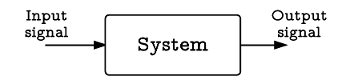
\includegraphics[width=0.6\textwidth]{img/system.png}
\end{figure}
\end{frame}

\begin{frame}[t]{Input-Output Relationship of Linear System}
\textbf{Linearity}:
\[ x_i[n] \mapsto y_i[n] \implies \sum_{i} \alpha_i x_i[n] \mapsto \sum_{i} \alpha_i y_i[n] \]
\end{frame}

\begin{frame}[t]{Input-Output Relationship of Time-Invariant System}
\textbf{Time-invariance}:  
\[ x_i[n] \mapsto y_i[n] \implies x_i[n - k] \mapsto y_i[n-k] \]
\end{frame}

\begin{frame}[t]{Linear Time Invariant (LTI) System}
\textbf{Input-Output Relationship}
\[ x_i[n] \mapsto y_i[n] \implies \sum_{i} \alpha_i x_i[n - k_i] \mapsto \sum_{i} \alpha_i y_i[n - k_i] \]
\end{frame}

\begin{frame}[t]{Importance of the Impulse Signal}
Any signal $x[n]$ can be represented as a linear combinration of time-shifted impulse signals.
\[ x[n]  = \sum_{k=-\infty}^{\infty} x[k] \delta[n - k] \]
\begin{figure}
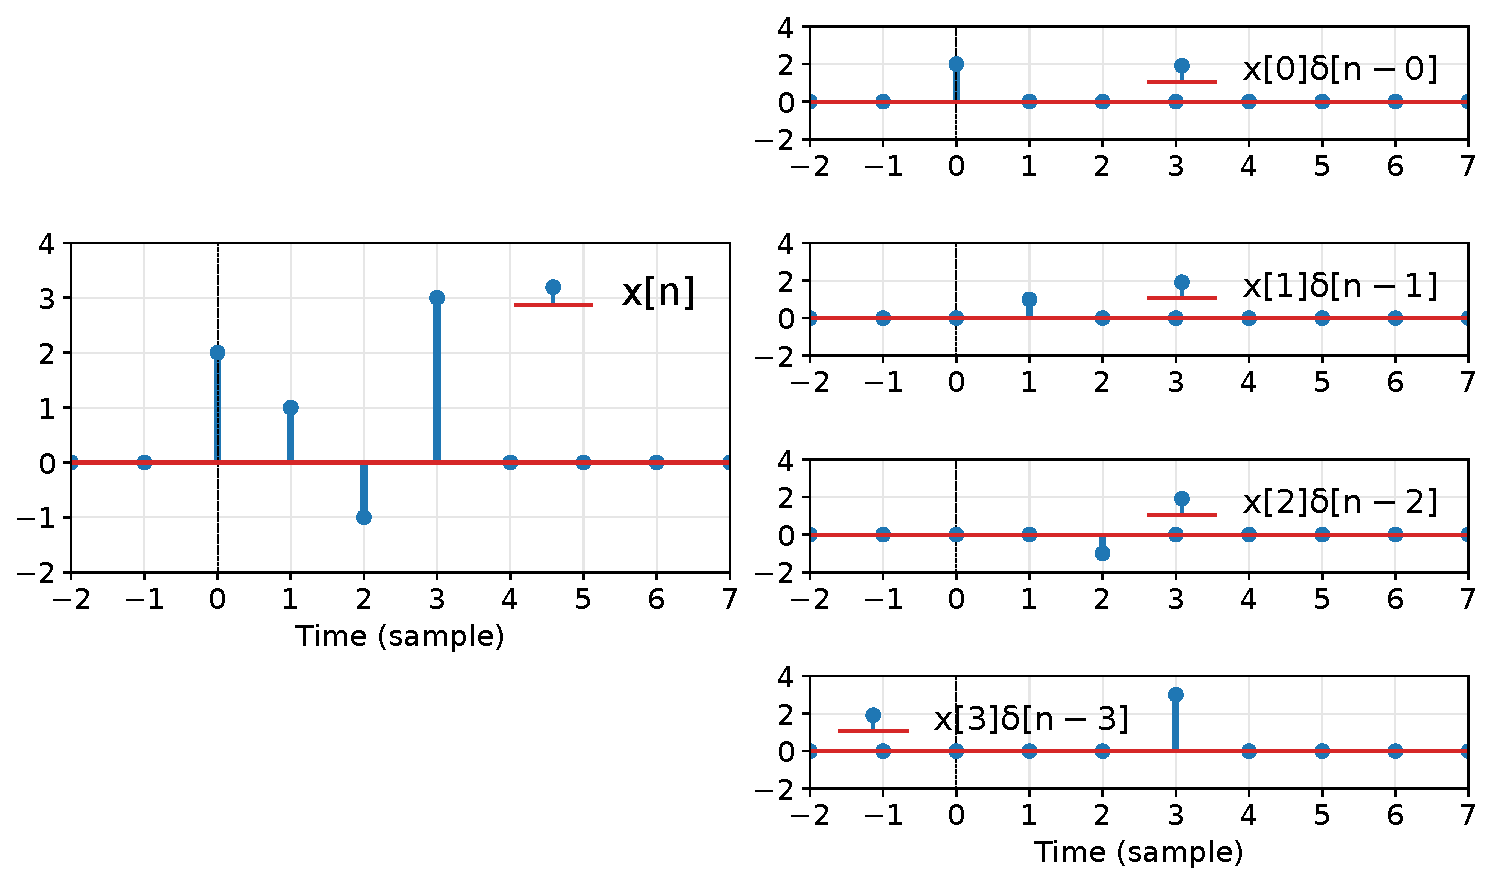
\includegraphics[width=0.6\textwidth]{img/sigimpdecomp.eps}
\end{figure}
\end{frame}

\begin{frame}[t]{Impulse Response of an LTI System}
\textbf{Impulse Response}: The response of an LTI system to an impulse input.

\[ h[n]  = \mathcal{H}\left( \delta[n] \right) \]

If we know this, then we know the following for an LTI system:
\[ \delta[n] \mapsto h[n] \implies \begin{cases}
\delta[n - k] &\mapsto h[n - k] \\
\alpha_k \cdot \delta[n - k] &\mapsto \alpha_k \cdot h[n - k] \\
\sum_k \alpha_k \cdot \delta[n - k] &\mapsto \sum_k\alpha_k \cdot h[n - k]
\end{cases} \]

\[ x[n] =\sum_k x[k] \cdot \delta[n - k] \xrightarrow{\quad \mathcal{H} \quad} \sum_k x[k] \cdot h[n - k] = x[n] * h[n] \]
\end{frame}

\begin{frame}[t]{Output of an LTI System}
\begin{figure}
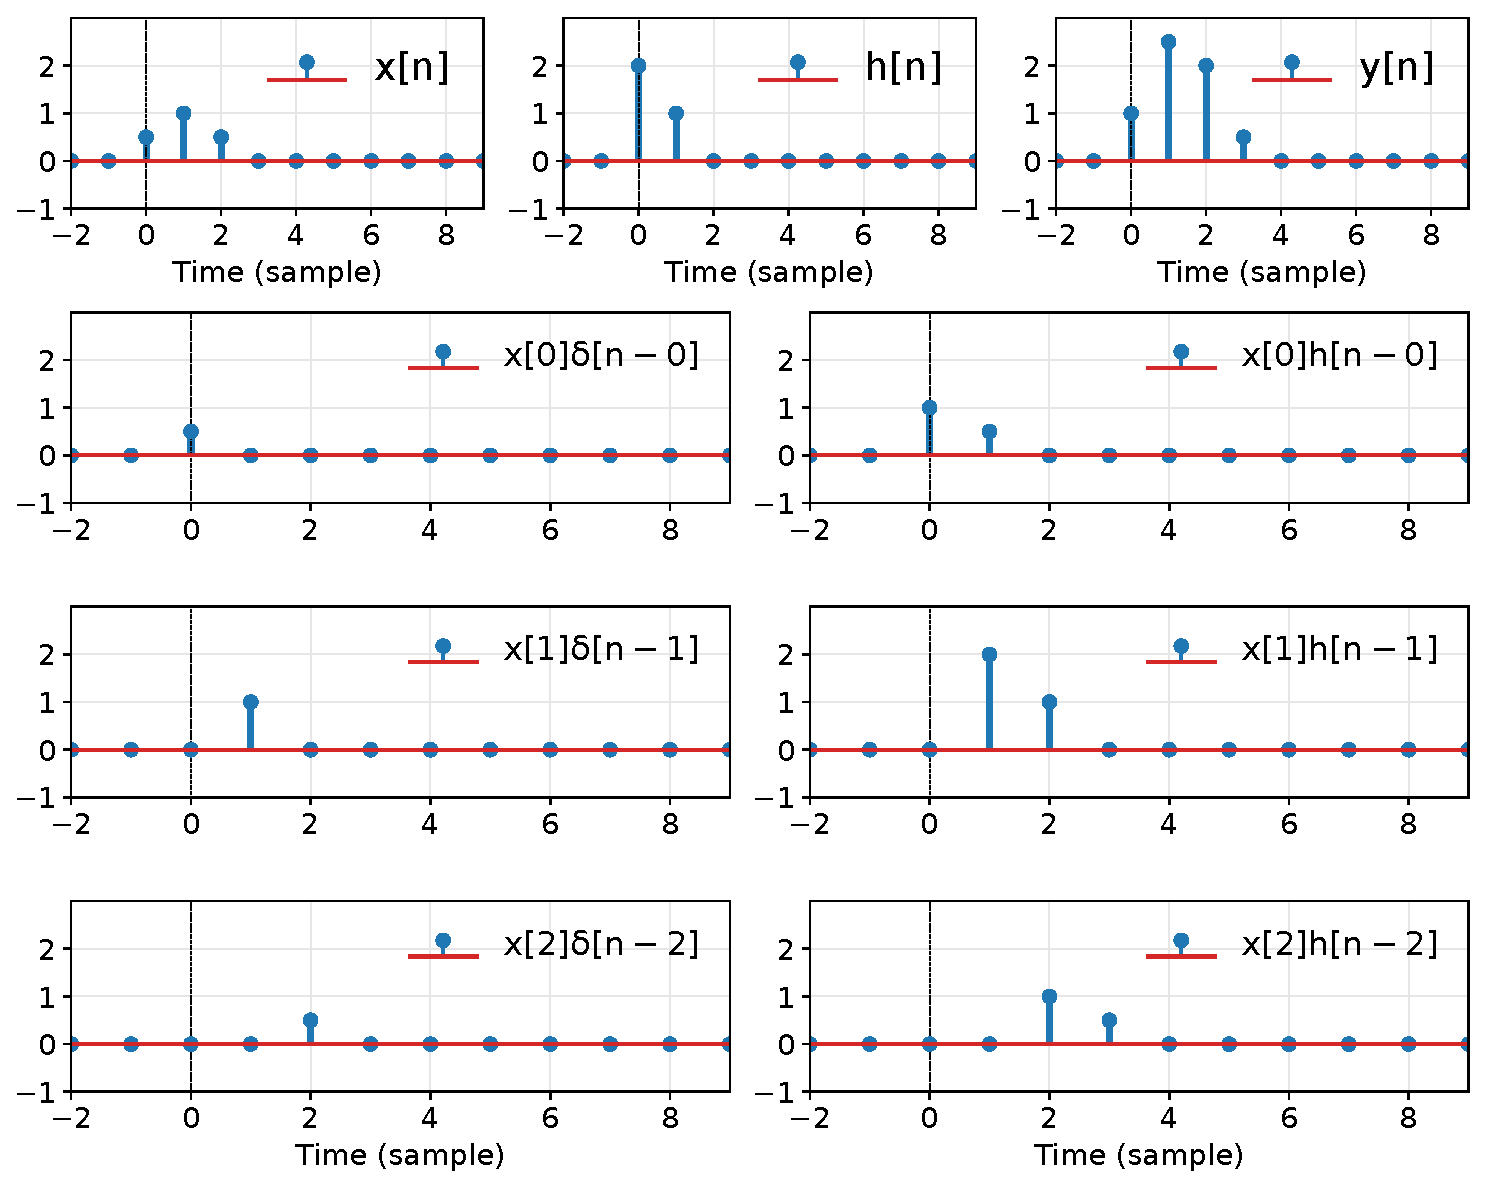
\includegraphics[width=0.6\textwidth]{img/convdemo1.eps}
\end{figure}
\end{frame}

\begin{frame}[t]{Convolution Sum}
\begin{Large}
\[ y[n] = x[n] * h[n] = \sum_k x[k] \cdot h[n - k] \]
\end{Large}
\end{frame}

\begin{frame}[t]{Alternative View of the Convolution Sum}
\begin{Large}
\[ y[n] = x[n] * h[n] = \sum_k x[k] \cdot h[n - k] \]
\end{Large}
\begin{center}
\begin{tabu}{c|c|c|c|c|c|c|c|c|c|c|c|c|c}
\hline
$k$ & $\cdots$ & -3 &  -2 & -1 & 0 & 1 & 2 & 3 & 4 & 5 & 6 & 7 & $\cdots$ \\ \hline
\rowfont{\color{red}} $x[k]$ & $\cdots$ & 0 & 0 & 0 & 0.5 & 1 & 0.5 & 0 & 0 & 0 & 0 & $\cdots$ &  \\ \hline
$h[\quad - k]$ & $\cdots$ &  &  &  &  &  &  &  &  &  &  &  & $\cdots$ \\ \hline
$h[\quad - k]$ & $\cdots$ &  &  &  &  &  &  &  &  &  &  &  & $\cdots$ \\ \hline
$h[\quad - k]$ & $\cdots$ &  &  &  &  &  &  &  &  &  &  &  & $\cdots$ \\ \hline
$h[\quad - k]$ & $\cdots$ &  &  &  &  &  &  &  &  &  &  &  & $\cdots$ \\ \hline
$h[\quad - k]$ & $\cdots$ &  &  &  &  &  &  &  &  &  &  &  & $\cdots$ \\ \hline
$h[\quad - k]$ & $\cdots$ &  &  &  &  &  &  &  &  &  &  &  & $\cdots$ \\ \hline
$h[\quad - k]$ & $\cdots$ &  &  &  &  &  &  &  &  &  &  &  & $\cdots$ \\ \hline
\end{tabu}
\end{center}
\end{frame}

\begin{frame}[t]{What does the impulse response tell us?}
\[
\begin{split}
y[n] &= x[n] * h[n] = \sum_k x[k] \cdot h[n - k] \\
     &= h[n] * x[n] = \sum_k h[k] \cdot x[n - k] \\
     &= \cdots + h[2] \cdot x[n-2] + h[1] \cdot x[n-1] \\
     &\quad \quad \,\,\, + h[0] \cdot x[n]\\
     &\quad \quad \,\,\, + h[-1] \cdot x[n + 1] + h[-2] \cdot x[n + 2] + \cdots
\end{split}
\]
\end{frame}

\begin{frame}[t]{Properties of convolution sum}
\begin{itemize}
  \item \textbf{Commutative}
  \[ x_1[n] * x_2[n] = x_2[n] * x_1[n] \]
  \item \textbf{Associative}
  \[ x_1[n] * \lp x_2[n] * x_3[n]\rp = \lp x_1[n] * x_2[n]\rp * x_3[n] \]
  \item \textbf{Distributive}
  \[ x_1[n] * \lp x_2[n] + x_3[n]\rp = x_1[n] * x_2[n] + x_1[n] * x_3[n] \]
  \item \textbf{Multiplicative identity}
  \[ x_1[n] * \delta[n] = x_1[n] \]
\end{itemize}
\end{frame}


\begin{frame}[t]{Impulse response, causality, and stability}
Let $h[n]$ be the impulse response of and LTI system $\mc{H}$. \vspace{0.5cm}

\begin{itemize}
  \item \textbf{Causaility}. The LTI system $\mc{H}$ is causal, if and only if,
  \[ h[n] = 0, \,\, \forall n < 0 \]
  \item \textbf{Stability}. The LTI system $\mc{H}$ is stable, if and only if,
  \[ \sum_{k=-\infty}^{\infty} \vert h[k] \vert < \infty \]
\end{itemize}
\end{frame}



\begin{frame}[t]{Interconnection of LTI systems}

\begin{figure}
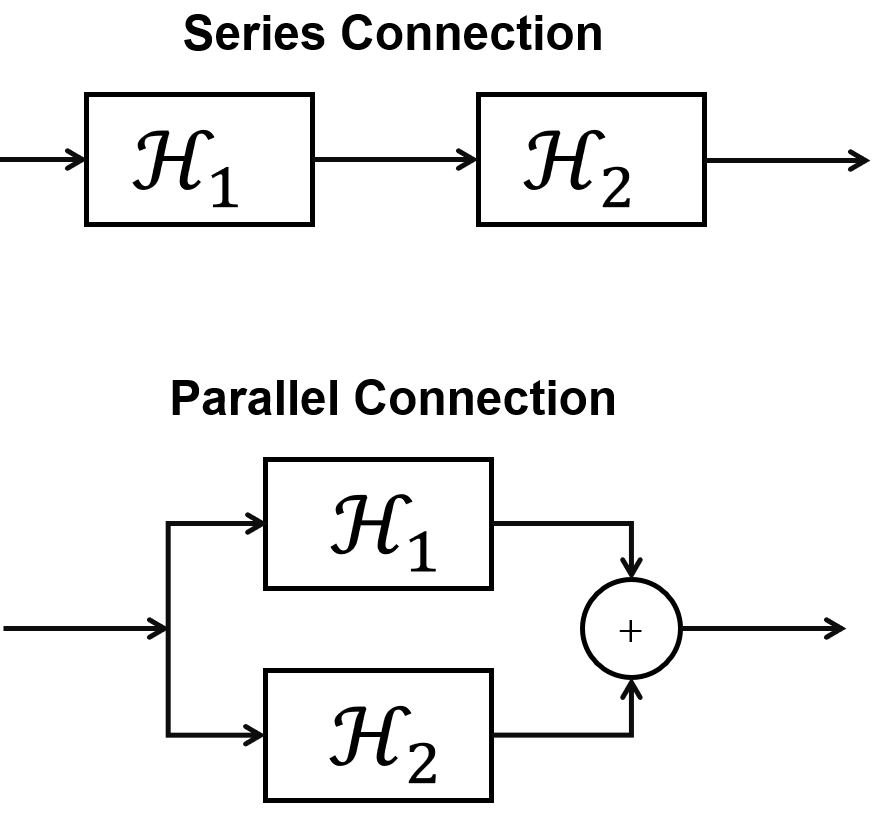
\includegraphics[width=0.5\textwidth]{img/connections.png}
\end{figure}

\end{frame}

\begin{frame}[t]{Finite and Infinite Impulse Response system}

Discrete-time LTI systems can be classified into two types based on the duration of the impulse response:
\begin{itemize}
  \item \textbf{Finite Impulse Response (FIR) system}. $h[n]$ is non-zero only for a finite duration of time, and it is uniformly zero outside this finite duration.
  \[ h[n] = 0, \,\, n < M_1 \,\, \text{and} \,\, n > M_2 \implies y[n] = \sum_{k=M_1}^{M_2} h[k]x[n-k] \]
\end{itemize}

Causality? \vspace{0.5cm}

Stability?


How would be implement this system?

\end{frame}


\begin{frame}[t]{Finite and Infinite Impulse Response system}

Discrte-time LTI system can be classified into two types of system based on the duration of the impulse response:
\begin{itemize}
  \item \textbf{Infinite Impulse Response (IIR) system}. $h[n]$ is of infinitely long  duration.,
  \[  y[n] = \sum_{k=-\infty}^{\infty} h[k]x[n-k] \]
\end{itemize}

Causality? \vspace{0.5cm}

Stability?

How would be implement this system?

\end{frame}

\begin{frame}[t]{Linear, constant-coefficient difference equations}
Consider the following system,
\[ y[n] = \sum_{k=0}^{\infty} x[n-k] \]

This system has a simple recursive form,
\[ y[n] = y[n-1] + x[n] \]
\end{frame}

\begin{frame}[t]{Linear, constant-coefficient difference equations}
A class of IIR systems can be expressed in recursive form through linear, constant coefficient difference equations,
\[ y[n] = -\sum_{k=1}^n a_k \cdot y[n - k] + \sum_{k=0}^{m} b_k \cdot x[n-k] \]

This allows us to implement such a system.
\end{frame}

\begin{frame}[t]{Linear, constant-coefficient difference equations}
A class of IIR systems can be expressed in recursive form through linear, constant coefficient difference equations,
\[ y[n] = -\sum_{k=1}^N a_k \cdot y[n - k] + \sum_{k=0}^{M} b_k \cdot x[n-k] \]

This allows us to implement such a system.
\end{frame}

\begin{frame}[t]{Linear, constant-coefficient difference equations}
Find the output of the system for $n \geq 0$ for the input $x[n] = u[n]$.
\[ y[n] = a_1 \cdot y[n - 1] + x[n] \]
\end{frame}

\begin{frame}[t]{Zero state and Zeo Input Responses of LTI system}
\[ y[n] = a_1 \cdot y[n - 1] + x[n] \longrightarrow \]

\textbf{Zero state response:} \vspace{2cm}


\textbf{Zero state response:} \vspace{2cm}
\end{frame}

\begin{frame}[t]{Linearity of a general recursive LTI system}
\[ y[n] = -\sum_{k=1}^N a_k \cdot y[n - k] + \sum_{k=0}^{M} b_k \cdot x[n-k] \]
\begin{enumerate}
  \item The total system response is the sum of the \textit{zero state} response and \textit{zero input} responses.
  \item The \textit{zero state} response satisfies the property of scaling and superposition.
  \item The \textit{zero input} response satisfies the property of scaling and superposition.
\end{enumerate}
\end{frame}

\begin{frame}[t]{Solution of linear constant coefficient difference equations}
\[ y[n] = -\sum_{k=1}^n a_k \cdot y[n - k] + \sum_{k=0}^{m} b_k \cdot x[n-k] \]
The general solution is given by (assuming the input is applied at time $n = 0$),
\[ y[n] = y_{h}[n] + y_p[n] \]
\begin{itemize}
  \item  $y_h[n]$ is the homogenous solution, i.e. the solution when the input is $0$.
  \item  $y_p[n]$ is the particular solution, i.e. the solution for the given input $x[n]$.
\end{itemize}
\end{frame}

\begin{frame}[t]{Homogenous Solution}
This is the solution to the following equation,
\[ y[n] + \sum_{k=1}^N a_k \cdot y[n - k] = 0\]
We are interested in the solution starting at $n=0$ with the initial conditions $\lc y[-1], y[-2], y[-3], \ldots, y[-N+1]\rc$.

\vspace{0.5cm} 

We first replace the term $y[n-k]$ to $z^{n-k}$, resulting in the following equation,
\[ z^n + \sum_{k=1}^N a_k \cdot z^{n - k} = 0 \implies z^N + a_1z^{N-1} + a_2z^{N-2} + \cdots + a_N = 0 \] 
\end{frame}


\begin{frame}[t]{Homogenous Solution}
\[ z^n + \sum_{k=1}^N a_k \cdot z^{n - k} = 0 \implies z^N + a_1z^{N-1} + a_2z^{N-2} + \cdots + a_N = 0 \]

Let $\lc \lambda_i \rc_{i=1}^N$ be the roots of the above polynominal equations, assuming there are $N$ distinct roots. Then, the homogenous solution has the following form,
\[ y_h[n] = C_1 \lambda_1^n + C_2 \lambda_2^n + C_3 \lambda_3^n + \ldots + C_N \lambda_N^n , \,\,\ n \geq 0 \]

The initial conditions can be used to solve for the constants $C_i$.
\end{frame}


\begin{frame}[t]{Homogenous Solution}
\[ z^n + \sum_{k=1}^N a_k \cdot z^{n - k} = 0 \implies z^N + a_1z^{N-1} + a_2z^{N-2} + \cdots + a_N = 0 \]

Let $\lambda_1$ by repeated $m$ times, then the homogenous solution has the following form,
\[ y_h[n] = \sum_{i=0}^{m-1} C_i n^i \lambda_1^n + \sum_{i=m+1}^N C_i \lambda_i^n , \,\,\ n \geq 0 \]

\end{frame}


\begin{frame}[t]{Particular Solution}
The particular solution $y_p[n]$ satisfies the following equation,
\[ y_p[n] + \sum_{k=1}^N a_k \cdot y_p[n - k] = \sum_{k=0}^{m} b_k \cdot x[n-k] \]

Based on the type of the input, we assume a particular form for the particular solution and solve for the constants in this solution to obtain the exact $y_p[n]$.

\begin{table}[]
\begin{tabular}{|c|c|}
\hline
Input Signal & Particular Solution \\ \hline
$A$ & $K$ \\ \hline
$u[n]$ & $K\cdot u[n]$\\ \hline
$\alpha^n$ & $K\cdot \alpha^n$\\ \hline
$n^p$ & $\sum_{i=0}^p K_i n^i$\\ \hline
$\cos \Omega n, \sin \Omega n$ & $K_1\cos \Omega n + K_2\sin \Omega n$\\ \hline
\end{tabular}
\end{table}
\end{frame}


\begin{frame}[t]{Example}
Find the output of the LTI system described by the following equation,.
\[ y[n] + 0.5 y[n-1] = x[n]; \quad x[n] = u[n], y[-1] = -2 \]
\end{frame}


\begin{frame}[t]{Example}
\end{frame}


\begin{frame}[t]{Example}
Find the output of the LTI system described by the following equation,.
\[ y[n] + y[n-1] -2 y[n-2] = x[n]; \quad x[n] = 0.1^n, y[-1] = 1, y[-2] = -1 \]
\end{frame}


\begin{frame}[t]{Example}
\end{frame}


\begin{frame}[t]{Impulse response of a Linear Time-invariant Recursive system}
\[ y[n] = -\sum_{k=1}^N a_k \cdot y[n - k] + \sum_{k=0}^{M} b_k \cdot x[n-k] \]

Impulse response is the \textit{zero state} response for the input $\delta[n]$. 

\vspace{0.5cm}
Find the impulse response of the following system,
\[ y[n] + 0.5 y[n-1] = x[n] + 2x[n-1] \]
\[ y[n] + y[n-1] - 2 y[n-2] = x[n] - x[n-1] \]
\end{frame}


\begin{frame}[t]{}
\end{frame}


\begin{frame}[t]{Impulse response of a Linear Time-invariant Recursive system}
\[ y[n] = -\sum_{k=1}^N a_k \cdot y[n - k] + \sum_{k=0}^{M} b_k \cdot x[n-k] \]

The impulse response has the general form,
\[ h[n] = \sum_{i=1}^{N} C_i \lambda_i^n \]

We solve for $C_i$ assuming zero initial conditions, $y[-1] = y[-2] = \cdots = y[-N+1] = 0$. \vspace{0.5cm}

The impulse response will be equal to the homogenous solution from $n = M + 1$, with the initial conditions $y[n-M], y[n-M-1], y[n-M-2], \ldots , y[n-M-N+1]$.
\end{frame}


\begin{frame}[t]{}
\end{frame}


\begin{frame}[t]{Exponential inputs to an LTI system}
Consider the following LTI system,
\[ y[n] = \sum_{k=-\infty}^\infty h[k] x[n-k] \]

If we apply an input $x[n] = z^n$, then we get
\[ y[n] = \sum_{k=-\infty}^\infty h[k] z^{n-k} = \lp \sum_{k=-\infty}^\infty h[k] z^{-k} \rp z^n = H\lp z \rp z^n \]
\end{frame}


\end{document}
